\documentclass{beamer}
\title{Gnidosz blotny}
\author{Dasher}
\date{\today}
\usepackage{amsfonts}
\usepackage[MeX]{polski}
\usepackage{graphicx}
\begin{document}
\frame{\titlepage}

\begin{frame}
	\frametitle{Spis Tresci}
	\tableofcontents
\end{frame}

\section{Gnidosz blotny}
\begin{frame}{Gnidosz blotny}
(Pedicularis palustris L.) --- gatunek nalezacy do rodziny zarazowatych. Wystepuje w Europie, na Kaukazie i w Kanadzie. W Polsce dosc czesty na calym nizu.
\begin{figure}
%\section{Kwiat}
\centering
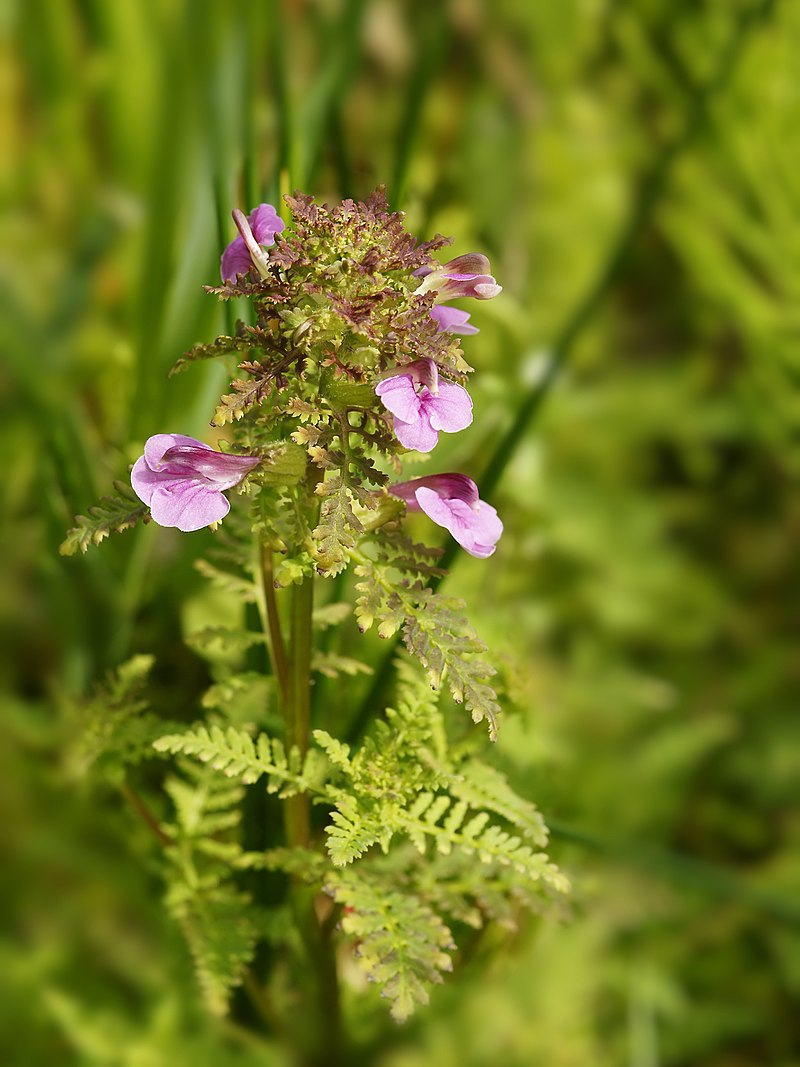
\includegraphics[width=0.25\hsize]{kwiat.jpg}
\caption{Gnidosz blotny}
\end{figure}
\end{frame}

\section{Morfologia}
\subsection{Lodyga}
\begin{frame}{Lodyga}
Wzniesiona, prosta, o wysokości 20---60 cm, gora rozgaleziajaca sie. Jest prawie naga, w srodku pusta.
\end{frame}

\subsection{Liscie}
\begin{frame}{Liscie}
Pierzastodzielne, o lancetowatych i karbowanych odcinkach, siedzace, zoltozielonego koloru.
\end{frame}

\subsection{Kwiaty}
\begin{frame}{Kwiaty}
Zebrane w luzne grono. Sa to kwiaty grzbieciste, wyrastaja w katach liści na krotkich szypulkach. Maja dwuwargowy rozdety kielich z pierzastowcietymi i odgietymi do tylu latkami. Jest to kielich trwaly, pozostający po przekwitnieciu. Purpurowa lub rozowa korona o rurce dluzszej od kielicha, orzesiona na bokach. Dolna warga zamyka wejscie do gardzieli korony, gorna, dwuzzbkowa warga jest scisnieta po bokach. 1 slupek, 4 dwusilne preciki ukryte pod gorna warga. Miodniki umieszczone u podstawy slupka, ale dostep do nich utrudniają wloski precikow.
\end{frame}

\subsection{Owoc}
\begin{frame}{Owoc}
Dwukomorowa, otoczona kielichem, okragla torebka.
\end{frame}

\subsection{Korzen}
\begin{frame}{Korzen}
Posiada ssawki, ktorymi wrasta w korzenie sasiadujacych roslin.
\end{frame}

\section{Biologia i ekologia}
\begin{frame}{Biologia i ekologia}
Roslina jednoroczna lub dwuletnia, hemikryptofit. Jest polpasozytem. Na uzytkowanych łakach uznawana za chwast, gdyz oslabia sasiednie rosliny wysysajac z nich wode i sole mineralne. Roslina miododajna, owadopylna, kwitnie od maja do lipca. Zapylana jest przewaznie przez trzmiele. Roslina trujaca.

Rosnie na mokrych lakach i torfowiskach. W gorach wystepuje po regiel dolny. W klasyfikacji zbiorowisk roslinnych gatunek charakterystyczny dla klasy (Cl.) Scheuchzerio-Caricetea nigrae.
\end{frame}

\section{Zmiennosc}
\begin{frame}{Zmiennosc}
Wystepuje w 2 podgatunkach:
\begin{itemize}
\item Pedicularis palustris L. subsp. opsiantha (Ekman) Almquist z Uznamu --- o koronie srednicy ok. 15 mm i rozgalezieniach lodygi o grubosci prawie rownej ich dlugosci.

\item Pedicularis palustris L. subsp. palustris
\end{itemize}
\end{frame}

\section{Zagrozenia i ochrona}
\begin{frame}
W latach 2004-2014 roslina byla objeta w Polsce scisla ochrona gatunkowa, od 2014 roku podlega ochronie czesciowej. Roslina zostala umieszczona w Polskiej Czerwonej Ksiegi Roslin jako gatunek narazony na wymarcie (kategoria zagrozenia VU). Te sama kategorie zagrozenia otrzymala w Czerwonej liscie roslin i grzybow Polski (2006, 2016). Zagrozeniem jest zanikanie stanowisk wynikające z osuszania terenów podmokłych i przeksztalcania ich w laki i inne tereny uzytkowe. Wiele stanowisk znajduje sie na obszarach chronionych, m.in. w Bialowieskim, Wielkopolskim i Tatrzanskim Parku Narodowym.
\end{frame}

\end{document}